\documentclass{article}
\usepackage{amssymb}
\usepackage{graphicx}
\usepackage{caption}
\usepackage{subcaption}
\usepackage{listings}
\usepackage{float} %figure inside minipage
\graphicspath{ {./images/} }
\usepackage[export]{adjustbox}
\usepackage{apacite}

\begin{document}

\section{Discontinuity in the PDE case}
\subsection{Introduction}
\label{subsection:pde_intro}
In this chapter, we present a similar investigation of solutions to problems with discontinuities in the partial differential equation (PDE) case. To that effect, we will use a 1D PDE epidemiological model similar to those often used in research in that area. 

Again, it is vital that numerical errors associated with the solvers are neglible compared to the modeling errors so that epidemiologist con perform conclusive errors. However, in the PDE case, we often find that rudimentary solvers (often a variation that reduce to using the Euler method) are used. As in the ODE case, it would be very suprising that these solvers are able to reach an accurate solution. To that effect, we spend Section $\ref{subsection:pde_software}$ on introducing BACOLIKR and explaining its importance for the accurate solving of PDE problems. To our knowledge, it is also the only PDE solver capable of event detection which as, shown in the previous chapter, becomes vital for accurate solutions of state-dependent discontinuity problems.

In Section $\ref{subsection:pde_thrashing}$, we reintroduce thrashing for the PDE case, in Section $\ref{subsection:pde_software}$, we provide the BACOLIKR description and in Section $\ref{subsection:pde_problem_def}$, we give a description of the epidemiological model used.

We provide a treatment of the time-dependent discontinuity problem with and without discontinuity handling in Section $\ref{subsection:pde_time_intro}$ and a treatment of the state-dependent discontinuity problem with and without event detection in Section $\ref{subsection:pde_state_intro}$.

\subsubsection{Thrashing in PDE models}
\label{subsection:pde_thrashing}
As was the case with ODE solvers, PDE solvers are also based on mathematical theories that guarantee convergence (a good solution) only when the solution and some of its higher derivatives are continuous. No rigorous mathematical theories guarantee that a PDE solver can solve a discontinuous problems but through experiments, it is known that $\emph{error-control}$ allows solvers to integrate through discontinuities. They do so by repeatedly reducing the step-size until the error of the new step satisfies the user-provided tolerance. Only then is the step accepted.

Thus, when a PDE solver is asked to integrate through a discontinuity, it thrashes. It repeatedly reduces the step-size at that discontinuity until the step-size is small enough to integrate through it. This is observed as a spike in the number of function evaluations at a discontinuity. Figure $\ref{fig:thrashing_pde}$ shows such a phenomenon. A problem with a discontinuity placed at t=30 is solved and we plot the cumulative number of function evaluation at each time interval that the solver, BACOLIKR takes. (We can clearly see the spike at t=30. )
 
\begin{figure}[H]
\centering
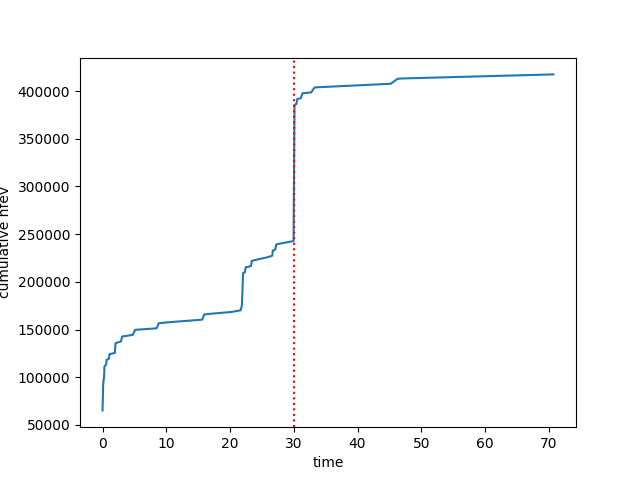
\includegraphics[width=0.7\linewidth]{./figures/pde_thrashing}
\caption{Thrashing in the PDE context}
\label{fig:thrashing_pde}
\end{figure}

In this chapter, we will show that PDE solvers with error-control, like BACOLIKR,  can integrate through one time-dependent discontinuity but that discontinuity handling lead to more efficient solutions as was the case with time-dependent dicontinuous ODE problems (See Section $\ref{subsection:pde_time_intro}$). We will also show that state-dependent discontinuity problems cannot be solved without event detection and that even with event detection, the user will have to be satisfied with an accuracy-efficiency trade-off (See Section $\ref{subsection:pde_state_intro}$).

\subsubsection{BACOLIKR, error-control event detection PDE solver}
\label{subsection:pde_software}
BACOLIKR is a member of the BACOL family of PDE solvers 8888 need reference 8888. Its underlying principle is the same a BACOL in that it solves PDE problems with a spline collocation method using the B-spline bases. 

The collocation process is applied on the spatial dimension to approximate the PDE system with a time-dependent larger ODE system. Using this ODE system and the provided boundary conditions, BACOLIKR produces a time-dependent system of Differential-Algebraic Equations (DAE) which it solves with the DAE solver, DASKR (a modification of DASSL with root-finding) 888 need a reference 888. DASSL provides adaptive time-stepping and adaptive method order selection (chooses an appropriate BDF method). BACOLIKR also provides control over the spatial error throug adaptive refinement of the spatial mesh. 

 
Being an error-control solver, BACOLIKR tries to satisfy a user provided tolerance in the most efficient way possible and by using a root-finding DAE solver like DASKR, BACOLIKR can also perform event-detection and thus can be used for cold starts around discontinuities. We emphasize these two qualities of BACOLIKR as they guarantee accuracy and efficiency that other implementations of PDE solvers, especially rudimentary ones, very rarely grant.

\subsubsection{Problem Definition}
\label{subsection:pde_problem_def}
In this paper, the PDE model we will try to solve is an extension of the SEIR model for epidemiological PDE studies that uses a spatial variable, x, and a time variable, t. Similar PDE models have been used before 8888 reference to PDE Cholera papers 8888 and either use the spread in geographical location or the spread across age groups as the additional spatial variable.

A PDE problem is fully described using a system of partial differential equations of the form:
\begin{equation}
u_t(x, t) = f(x, t, u(x,t), u_x(x,t), u_{xx}(x,t))
\end{equation} 
over a spatial domain ${a \leq x \leq b}$ and an initial time ${t_0}$. 

It requires a set of initial conditions of the form:
\begin{equation}
u(x, t) = u_0(x)
\end{equation}
for x in the spatial domain, ${a \leq x \leq b}$.

It also requires boundary conditions of the form:
\begin{equation}
b_L(t, u(a,t), u_x(a,t)) = 0, b_R(t, u(b,t), u_x(b,t)) = 0 
\end{equation} 
for every time, $t \geq t_0$ .

To that effect, we define an SEIR model based on the one developed by Andrew Fraser 88888 Reference 88888 as follows:

The system of PDEs is:
\begin{equation}
S(x, t)_t = D_S(x)S(x, t)_{xx} + \mu N - \mu S(x, t) - \frac{\beta}{N}S(x, t)I(x, t)
\end{equation}
\begin{equation}
E(x, t)_t = D_E(x)E(x, t)_{xx} + \frac{\beta}{N}S(x, t)I(x, t) - \alpha E(x, t) - \mu E(x, t)
\end{equation}

\begin{equation}
I(x, t)_t = D_I(x)I(x, t)_{xx} + \alpha E(x, t) - \gamma I(x, t) - \mu I(x, t)
\end{equation}

\begin{equation}
R(x, t)_t = D_R(x)R(x, t)_{xx} + \gamma I(x, t) - \mu R(x, t)
\end{equation} 

The spatial domain is $-5 \leq x \leq 5$ and the temporal domain is $0 \leq t \leq 70$ for the time-dependent discontinuity problem but we will use $0 \leq t \leq 200$ for the space-dependent discontinuity problem as we attempt a long-term forecast.

The parameters for the SEIR are as such: $\mu$, the birth rate, is set to $\frac{0.01}{365}$. $\gamma$, the recovery rate is 0.06, $\alpha$, the incubation rate is 0.125 and we will vary the transmission rate, $\beta$, between 0.035 and 0.9 based on whether measures, such as social distancing and others, are implemented or not in the model. The population size, N, is $37*10^{6}$.

The model also uses diffusion functions $D_S(x)$, $D_E(x)$, $D_I(x)$ and $D_R(x)$ to start the infection at a specific point in the spatial domain and spread it over time. These are as follows:
\begin{equation}
D_S(x) = D_E(x) = D_R(x) = (maxD_s - minD_s)e^{-10(\sqrt{x^{2}} - 1)^2)} + minD_s
\end{equation} 
\begin{equation}
D_I(x) = D_E(x)/10
\end{equation}
The diffusivity parameters $maxD_s$ and $minD_s$ are 0.8 and 0.01 respectively. 

\begin{figure}[H]
\centering
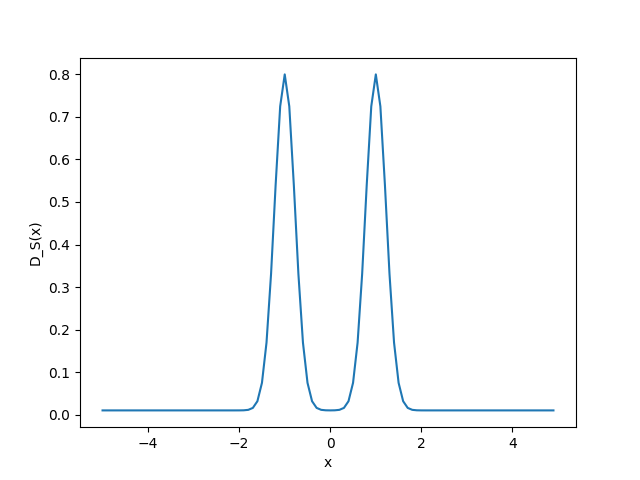
\includegraphics[width=0.7\linewidth]{./figures/pde_D_s}
\caption{Plot of the diffusivity parameter $D_S(x)$}
\label{fig:pde_D_s}
\end{figure}

The set of initial conditions are defined over the spatial domain as such:
\begin{equation}
S(x, 0) = N - I(x, 0)
\end{equation}
\begin{equation}
I(x, 0) = 100e^{-x^2}
\end{equation}
\begin{equation}
E(x, 0) = R(x, 0) = 0
\end{equation}

\begin{figure}[H]
\centering
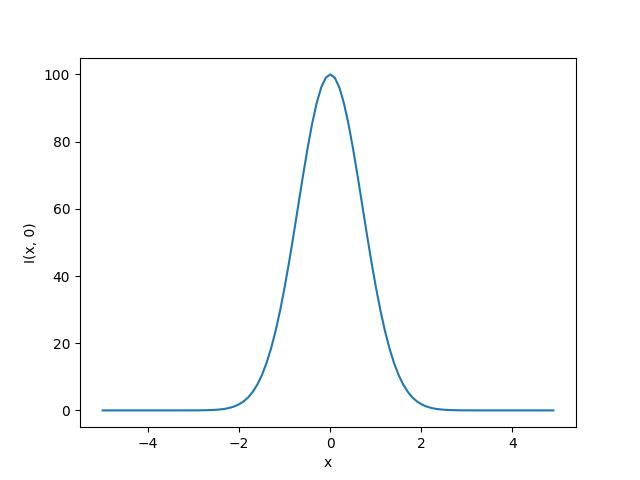
\includegraphics[width=0.7\linewidth]{./figures/pde_I_0}
\caption{Plot of the initial condition I(x, 0)}
\label{fig:pde_I_0}
\end{figure}

We will use the default boundary conditions 888888888888888888 I did not understand what BACOLIKR is doing for the initial conditions here 888888888888888888

The above gives us a complete PDE problem definition. To this problem we will add discontinuities as follows: 
In the time-dependent discontinuity problem (Section $\ref{subsection:pde_time_intro}$), we will integrate the model with $\beta$ at a value of 0.9 from t=0 to t=30, we will then change the value of $\beta$ to 0.035 and integrate until t=70. This change in the parameter introduces a discontinuity. This simulates a scenario where 30 days into a disease, measures are introduced to slow its spread.

In the state-dependent discontinuity problem (Section $\ref{subsection:pde_state_intro}$),, we start the integration with the value of $\beta$ at 0.9 until the integral value of the E-component of the solution over the spatial domain at a specific time-step is 30000. When that integral value reaches 30000, we change the value of $\beta$ to 0.035 until the integral value of the E-component over the spatial domain reaches 10000. We then integrate with a value $\beta$ of 0.9. We repeat this process until t=200. This process simulates a series of introducing and relaxing measures, such as social distancing, based on the total number of exposed individuals across the whole region.

\subsection{Time Dependent Discontinuity}
\label{subsection:pde_time_intro}
In this section, we investigate the thrashing experienced by BACOLIKR on the SEIR model with a time-dependent discontinuity. 

The time dependent discontinuity is introduced by changing the value of SEIR modelling parameter, $\beta$ from 0.9 to 0.035 at t=30.

We note that this section demonstrates that the PDE time-dependent discontinuity is similar to the ODE time-dependent discontinuity problem. We will show that accurate solutions can be found without the use of discontinuity handling (to eye-level accuracy) but that the use of a cold start drastically improves the efficiency.

For the following sections, we will plot the E-component of the solution at x=0 to show both that  the problem has an exponentially growing component and the rapid change to exponential decay as the parameter $\beta$ changes.

\subsubsection{Naive treatment of the time-dependent discontinuity PDE model}
\label{subsubsection:pde_time_naive}
The naive treatment for time-dependent discontinuities is to use if-statements in the right-hand side function itself using the time argument.

For our model, we use the time argument to say that the integration starts with a value of $\beta$ at 0.9 and that from t=30 onwards, the value for $\beta$ is 0.035. The pseudo-code for this approach is as follows:

\begin{minipage}{\linewidth}
\begin{lstlisting}[language=Python]
function model_with_if(t, x, u, ux, uxx)
    // ...
    beta = 0.9
    if t >= 30:
        beta = 0.035
    // ...
    return (dSdt, dEdt, dIdt, dRdt)

\end{lstlisting}
\end{minipage}

This change in the $\beta$ parameter introduces a discontinuity in the model, which leads to thrashing as discussed in Section $\ref{subsection:pde_thrashing}$ as the assumptions of continuity of the function and its derivatives no longer hold. However as we have shown in Section 8888 Refer to naive ODE time problem 8888 for the ODE case, error-control PDE solvers can also reduce the step-size extensively to integrate through one discontinuity. (See Figure $\ref{fig:pde_time_disc_naive}$.)


\begin{figure}[H]
\centering
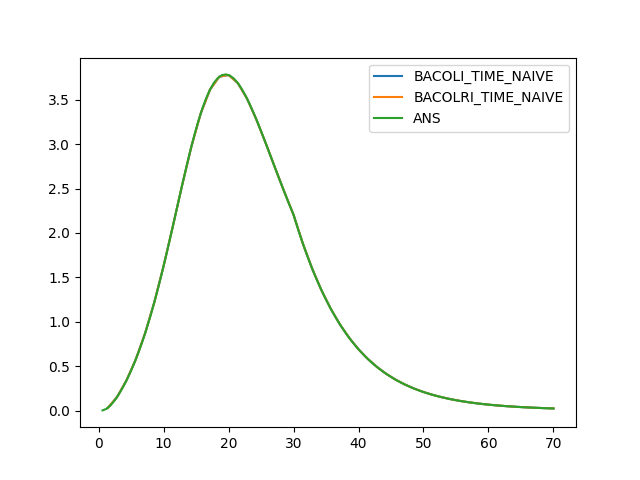
\includegraphics[width=0.7\linewidth]{./figures/pde_time_disc_naive}
\caption{Naive treatment of time discontinuity (at tolerance of $10^{-6}$)}
\label{fig:pde_time_disc_naive}
\end{figure}

From Figure $\ref{fig:pde_time_disc_naive}$, we can see that to eye-level accuracy, the results are accurate. We will now show how a cold start can give the same level of accuracy while using less function evaluations and thus being more efficient.

\subsubsection{Discontinuity handling to solve the time-dependent PDE model}
\label{subsubsection:pde_time_disc_hand}
In this section, we discuss the use of discontinuity handling through cold starts as it pertains to PDE problems. Though the error-controlled solver, BACOLIKR, were able to get accurate solutions, we will show that cold starts allow it to be more efficient.

We re-iterate that a solver is said to perform a cold start when it restarts the integration by using the last previously obtained solution as the initial value for the next step. The solver must clear all its data structures, start with a new spatial mesh, start with a new initial step-size and start with the default order. This way the solver does not allow any results from previous steps to interfere with the next step. Modern PDE solvers like BACOLIKR have several flags that a user can set along the integration to perform cold starts. We will use this flag to improve the efficiency of our solutions.

The idea is to integrate up to the discontinuity, cold start at the discontinuity and integrate past the discontinuity with the new model. In our case, we integrate the problem with one call from t=0 to t=30 with the model function using 0.9 as the $\beta$ parameter. We then set up a cold start and integrate from t=30 to the end of the time interval with another call to the solver. The pseudo-code for this approach is as follows

\begin{minipage}{\linewidth}
\begin{lstlisting}[language=Python]
function model_before(t, x, u, ux, uxx):
    // ...
    beta = 0.9
    // ...
    
function model_after(t, x, u, ux, uxx):
    // ...
    beta = 0.035
    // ...

solution = pde_solver.init(...)

tspan_before = [0, 30]
pde_solver(solution, model_before, tspan_before)

solution.cold_start_flag = True

tspan_after = [30, 70]
pde_solver(solution, model_after, tspan_after)

\end{lstlisting}
\end{minipage}

\begin{figure}[H]
\centering
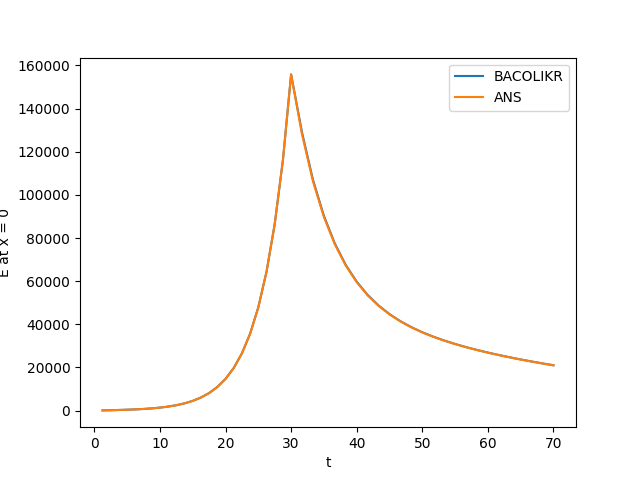
\includegraphics[width=0.7\linewidth]{./figures/pde_time_disc_disc_hand}
\caption{Discontinuity handling for time discontinuity problem (at tolerance of $10^{-6}$)}
\label{fig:pde_time_disc_disc_hand}
\end{figure}

As expected, Figure $\ref{fig:pde_time_disc_disc_hand}$ shows that BACOLIKR with the cold start was able to provide a solution with the same eye-level accuracy as it did without the cold start.
We now note that the use of a cold start required the solver to make 359, 755 function evaluations whereas the solver without this cold start required 417505 function evaluations. We were thus able to make 50000 less function evaluations which gives around a $14\%$ gain in efficiency.

\subsubsection{PDE Time-dependent discontinuity problem tolerance study}
\label{subsubsection:pde_time_tol}

As is the case with ODE research, a researcher might want to coarsen the tolerance of the solver if they need to run the solver in a loop or through an optimisation algorithm (See Appendix 8888 point to Althaus Ebola paper 8888). So we now perform a tolerance study on this time-dependent discontinuity problem to see whether the discontinuity handling allows us to use coarser tolerances as it did in the ODE case. We will also solve the problem at sharper tolerances to show how the use of discontinuity handling drastically improves the efficiency.

Figures $\ref{fig:pde_time_disc_bacolikr_naive_tol}$ shows the accuracy of the solutions without discontinuity handling at the different tolerances while Figure $\ref{fig:pde_time_disc_bacolikr_disc_hand_tol}$ shows the solutions with discontinuity handling at the different tolerances.
\begin{figure}[H]
\centering
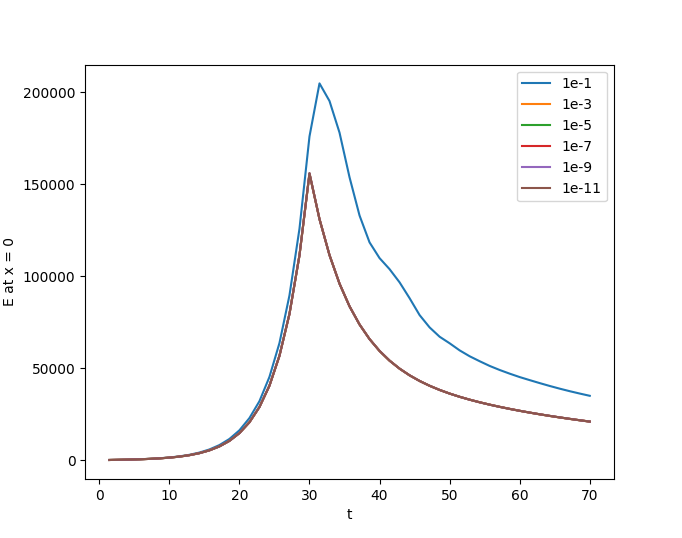
\includegraphics[width=0.7\linewidth]{./figures/pde_time_disc_bacolikr_naive_tol}
\caption{Time dependent discontinuity tolerance study with BACOLIKR without discontinuity handling}
\label{fig:pde_time_disc_bacolikr_naive_tol}
\end{figure}

\begin{figure}[H]
\centering
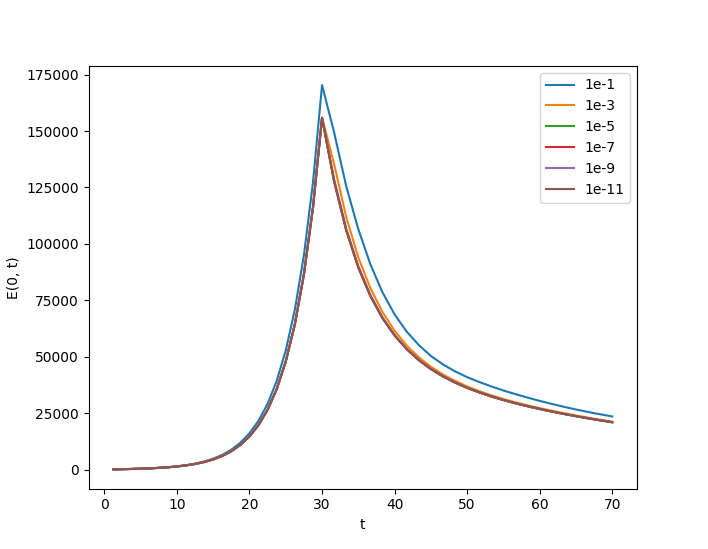
\includegraphics[width=0.7\linewidth]{./figures/pde_time_disc_bacolikr_disc_hand_tol}
\caption{Time dependent discontinuity tolerance study with BACOLIKR using discontinuity handlng}
\label{fig:pde_time_disc_bacolikr_disc_hand_tol}
\end{figure}

We note that both in the case with discontinuity handling and the case without it, the solutions at $10^{-1}$ are inaccurate. We note that surprisingly, the solution at $10^[-3]$ is more accurate without discontinuity handling than with. We explain this fact by noting that the step-size at $10^{-3}$ was much smaller than required in the case with discontinuity handling than in the case without. Thus though the solution is more accurate, the solver is being inefficient as it could satisfy this tolerance with a much smaller step-size. This can be see in Table $\ref{tab:pde_time_nfev}$ where we can see that it is doing around 2500 more function evaluations than required. As for all the tolerances sharper than $10^{-3}$, the solutions are all eye-level accurate.

\begin{table}[h]
\caption {PDE time discontinuity tolerance study} 
\label{tab:pde_time_nfev}
\begin{center}
\begin{tabular}{ c c c  } 
tolerance & BACOLIKR naive nfev & BACOLIKR disc hand nfev \\ 
1e-1      &   40, 800           &   55, 400   \\
1e-3      &   79, 220           &  76, 750    \\
1e-5      &  206, 980           &  208, 870    \\
1e-7      &  733, 210           &  543, 850     \\
1e-9      & 1, 904, 080         & 1, 653, 830   \\
1e-11     & 7, 140, 875         & 4, 979, 555   \\
\end{tabular}
\end{center}
\end{table}

Table $\ref{tab:pde_time_nfev}$ shows how more efficient the use of discontinuity handling is. We note that the lower count of the number of function evaluation for the case without discontinuity handling at a tolerance of $10^{-1}$ can be ignore as the solutions at this tolerance at very inaccurate. We then note that for any sharper tolerance, the use of discontinuity handling is a gain in efficiency and that at very sharp tolerance such as $10^{-11}$, the solver does around 2 million less function evaluations with a cold start than without (around a $30\%$ gain in efficiency). 

\subsection{State Dependent Discontinuity}
\label{subsection:pde_state_intro}
In this section, we discuss a state-dependent discontinuity problem. Again, we note that state-dependent discontinuity problems are not as trivial as time-dependent discontinuity problems and that in those problems, we do not have a trivial way to do a cold start programmatically. We will also attempt a long term forecast in this section as we will run the solver to t=200 to see for how long the solver can provide accurate solutions.

In state-dependent discontinuity problems, we use the value of one or several components of the solution to dictate how the model should behave. We compare the solution component(s) against predetermined thresholds and if these thresholds are crossed, we change the model equation. However, unlike, in the ODE case, in the PDE case we have another dimension to account for, the spatial dimension. Some of the ways to do so are listed below:
\begin{itemize}
\item Pick a spatial value, say x = 0, and sample the state value at this spatial point at every time interval. If the state value meets a certain threshold, we apply a different model, else we use the same model

\item Find some statistic measure (min, max, mean, median) across the spatial domain and use that value for the comparison with the threshold.

\item Integrate over the spatial domain and use that integral value for the comparison against the threshold. Essentially this does a `sum' across the spatial domain of the solution component.
\end{itemize}

In this report we will use the third method in that we will integrate over the spatial domain. If the value of the integral crosses a maximum threshold (30000) while measures are not implemented, the value of the parameter $\beta$ is changed from 0.9 to 0.005 and if measures are implemented and we cross a certain minimum threshold (10000), the value of the parameter $\beta$ is changed back to 0.9. 

Again, we note that a discontinuity is introduced by the change in the parameter $\beta$, as the right-hand side function is essentially changed to another one, and thus a discontinuity is introduced no matter which of the method presented above, a researcher might use to account for the spatial dimension.
 
For the following sections, we will plot the integral value of the E-component over the spatial dimension per time. An accurate solution would thus look like a graph oscillating cleanly between 10000 and 30000 as the models are changed.
\subsubsection{Naive treatment of the state-dependent discontinuity model}
\label{subsubsection:pde_state_naive}
The naive treatment of this problem involves using global variables which are toggled based on the integral value over the spatial domain to denote which model to use. 

In our case we can use a global boolean variable to say whether measures are implemented or not. This global variable is toggled to true when it was previously false and we reached an integral value of 30, 000 over the spatial domain, indicating that the number of exposed individual is high and that measures will now be implemented, and is toggled to false when it was previously true and the number of exposed individual is now 10, 000 across the spatial domain, indicating that the measures will be relaxed. When measures are implemented, the value of $\beta$ is 0.035 while when measures are not implemented the value of $\beta$ is 0.9.

In the naive implementation, the user will have to pick the time steps at which the solver should stop and run an integration over the spatial domain to get a value to compare against the thresholds. This form of manual time stepping introduces another parameter, the `number of time intervals', that the user will have to fine-tune to obtain accurate results. We will show, in this and the next section why this parameter is very hard to get right despite how crucial it is to get accurate results. If the variable is too small, we will toggle the global variable too late as we will check the integral value after it had already crossed the threshold and if the variable is too big, we will check the integral value too often which will reduce the efficiency. 

The naive approach in our case will be to divide the time domain into $num\_time\_intervals$ equal intervals. At the end of each interval, the solver will make use of an interpolant over the spatial domain to integrate it the E-component of the solution using a compound trapezoidal rule. This integral value will be compared against the threshold and thus if measures are not implemented and the integral is greater than 30, 000, the maximum threshold, the global variable indicating that measures are implemented will be switched to true to set the parameter $\beta$ to 0.035. When there are no measures implemented and the integral value less than 10, 000, the minimum threshold, the global variable is switched to false indicating that $\beta$ is now at 0.9 as measures are relaxed. The pseudo-code for this approach is as shown:

\begin{minipage}{\linewidth}
\begin{lstlisting}[language=Python]
measures_implemented = False

function model(t, x, u, ux, uxx):
    // ...
    global measures_implemented
    if (measures_implemented):
    		beta = 0.035
    	else:
    		beta = 0.9
    // ...

tstart = 0
tstop = 200
num_time_intervals = 400
time_step_size = (tstop - tstart) / num_time_intervals
solution = pde_solver.init()

t_current = tstart
t_next = t_current + time_step_size

while t_current < tstop:
	tspan = [t_current, t_next]
	pde_solver(solution, model, tspan)
	
	integral_value = integrate( spatial_interpolate(solution) )
	
	if (not measures_implemented):
		if (integral_value >= 30000):
			measures_implemented = True
	else:
		if (integral_value <= 10000):
			measures_implemented = False
	
	t_current = t_next
	t_next = t_next + time_step_size
\end{lstlisting}
\end{minipage} 

===========================================================
Now that we are using BACOLIKR, we can look to do a cold start even in the naive implementation
basically, every time we switch the global variable, we can also set the cold start flag...
Tell me if you want me to add this. I think this might add around 3-5 more pages.... 
===========================================================

Figure $\ref{fig:pde_state_disc_naive_400vs1000}$ shows integral value with 400 time intervals and 1000 intervals over the time period alongside a highly accurate solution obtained via event detection at sharp tolerance. We can see how both solutions are wrong as none are aligned with the `answer'. In the next section, we will show why the naive implementation cannot arrive at an accurate solution and in the section after that, we will show how event detection provide a more intuitive way to solve such problem.

\begin{figure}[H]
\centering
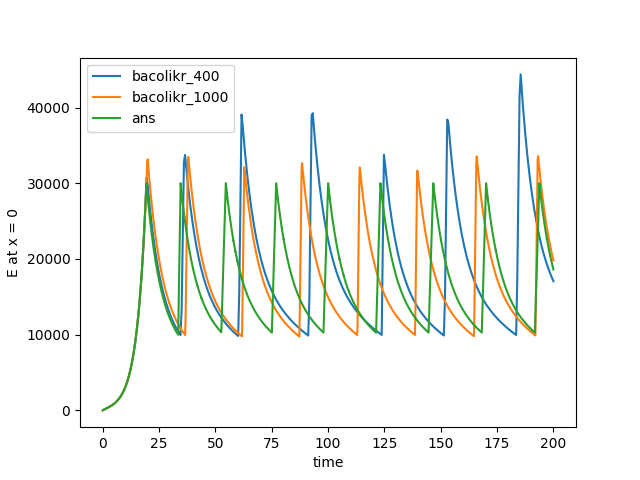
\includegraphics[width=0.7\linewidth]{./figures/pde_state_disc_naive_400vs1000}
\caption{Integral value plot of naive treatment to the state-dependent discontinuity problem at a tolerance of $10^{-6}$ using 400 vs 1000 time intervals}
\label{fig:pde_state_disc_naive_400vs1000}
\end{figure}

\subsubsection{Why the naive method cannot give an accurate solution}
\label{subsubsection:pde_state_naive_always_inaccurate}
The naive method cannot solve the problem accurately because of the problem of choosing a correct number of time intervals. The integration routine and the check is only performed after the threshold has been crossed and not exactly at the point of crossing. This means that we may take up to one additional time step with the previous $\beta$ value and not the correct one.

One idea to solve this problem would be to use an exceedingly large number of time intervals (10000 in our case) such that we take the smallest step possible with the old value. Figure $\ref{fig:pde_state_disc_naive_1000vs10000}$ shows how doing so produces a solution more in line with the high accuracy event-detection solution. However even this plot does not approach the accurate solution, especially at the later times. 

We could now use an even larger number of time intervals but this process of finding the optimal number of intervals is not intuitive. Using a high number of intervals will lead to a lost in efficiency as we will have to run the integration routine too often. Manually fine-tuning the number of time intervals variable is thus not the optimal way of solving this problem. 

Our only option is to use event detection. In the next section, we will show how event detection provide an intuitive, efficient and accurate way of solving such problems. It will allow us to correctly cold start when needed and thus have BACOLIKR integrate only on continuous sub-problems of the state-dependent discontinuity problem. It will also find the exact time at which the integral crosses a threshold and it will run the integration routine the minimum number of times needed to obtain an accurate solution, improving the efficiency of the solver as well.

\begin{figure}[H]
\centering
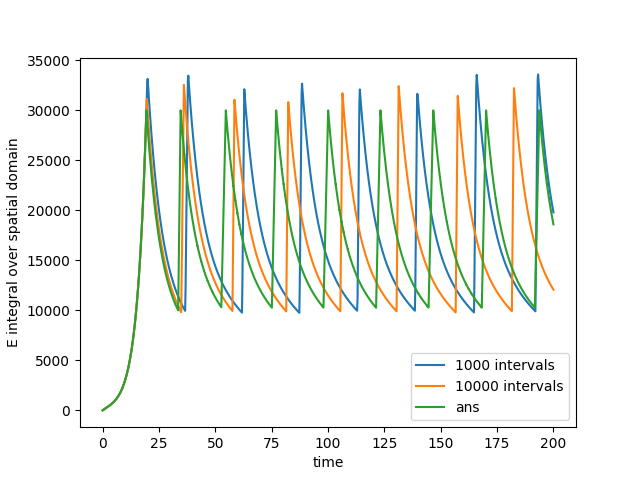
\includegraphics[width=0.7\linewidth]{./figures/pde_state_disc_naive_1000vs10000}
\caption{Integral value plot of naive treatment to the state-dependent discontinuity problem at a tolerance of $10^{-6}$ using 1000 vs 10000 time intervals}
\label{fig:pde_state_disc_naive_1000vs10000}
\end{figure}

\subsubsection{Event Detection solution to the naive state-dependent discontinuity model}
\label{subsubsection:pde_state_event_detection}
In the previous section, we have explained the problem with using manual time-stepping to obtain an accurate solution. In this section, we will present event detection in the PDE case, explain how it leads to more accurate results, explain how it makes the minimum number of calls to the integration routine required to obtain an accurate solution and will also discuss solutions to the problems that arise in using event detection to solve state-dependent discontinuity problems.

As is the case with ODE solvers, event detection is also present in some PDE solvers. Event detection also works in the same way as it does in the ODE case. To use event detection, the user provides a root function to the PDE solver. The root function uses the spatial mesh and the solution over the previously completed time step to return a floating point number. A root is detected when that floating point number is 0. After each time step, the solver calls the root function with the solution at the current time step alongside the current spatial mesh and some other information and stores its return value. If the return value returned by the root function changes sign between two consecutive steps, a root is present in between the steps. The PDE solver will then employ a root-finding routine within the time-step to find where the root function is zero. The solver then returns, setting flags indicating that it has found a root and provides the values and other information about the solution at the root.
 
BACOLIKR is an improvement to the BACOLI solver of the BACOL family of 1D PDE solvers (Give refernece) which has root finding capabilities. Instead of using DASSL as its DAE solver, it uses DASKR which can detect roots as it solves a DAE system.   

To solve the state-dependent discontinuity function, we define two pairs of root and model functions. One pair is to be used when integrating when there are no measures in place. The model function will have the variable $\beta$ at a value of 0.9 and the root function will do the integration of E-component of the solution over the spatial domain at the current time step and will return if the integral value is close to the maximum threshold. 30, 000. The second pair will have a model function with $\beta$ at a value of 0.035 and the root function looking for a root at 10, 000. The solver starts with the first pair as measures are not implemented. It will then return when the 30000 threshold is met. At this point we will set the cold start flag and run the solver with the second pair of model-root functions. The solver will now return when the integral value of the E-component crosses 10, 000. When that happens, we cold start again and run the solver with the first model-root function pair. We repeat this process until the solver reaches t=200. The pseudo-code for this approach is as follows:

\begin{minipage}{\linewidth}
\begin{lstlisting}[language=Python]
function model_no_measures(t, x, u, ux, uxx):
	// ...
	beta = 0.9
	// ...
	
function root_max_value(t, solution):
	// ...
	integral_value = integrate(interpolate(solution))
	return integral_value - 30000
	
function model_with_measures(t, x, u, ux, uxx):
	// ...
	beta = 0.035
	// ...
	
function root_min_value(t, solution):
	// ...
	integral_value = integrate(interpolate(solution))
	return integral_value - 10000

tstart = 0
tstop = 200
t_current = tstart
measures_implemented = false

while t_current < tstop:
	tspan = [t_current, t_stop]
	if (measures_implemented):
		pde_solver(solution, model_with_measures, 
			tspan, root_min_value)
	else:
		pde_solver(solution, model_no_measures, 
			tspan, root_max_value)
		
	if (solution.root_flag == True):
		solution.cold_start_flag = True
		// switch model-root pair
		measures_implemented = not measures_implemented
	
	t_current = solution.t

\end{lstlisting}
\end{minipage}

Figure $\ref{fig:pde_state_disc_event_tol_6}$ shows the solution at a tolerance of $10^{-6}$ of using event detection on the state-dependent discontinuity problem. We can see that the solution correctly oscillates between 10, 000 and 30, 000 and that for the first few oscillations, it lines up with the highly accurate solution. We then see that though it oscillates correctly, at the later times, it is not aligned with the highly accurate solution especially at the roots. 

\begin{figure}[H]
\centering
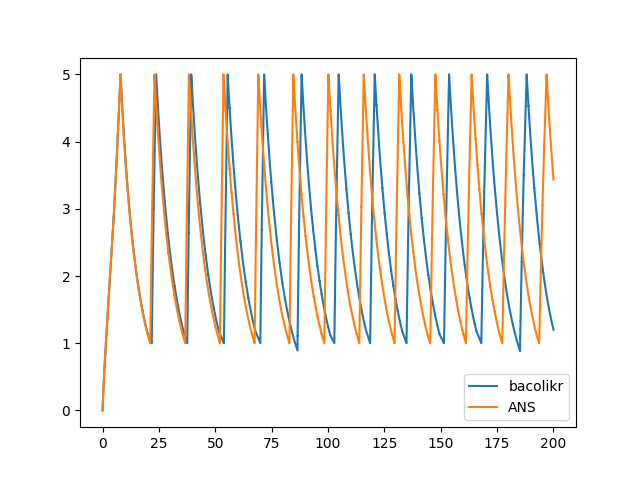
\includegraphics[width=0.7\linewidth]{./figures/pde_state_disc_event_tol_6}
\caption{Integral value plot of the event detection solution to state-dependent discontinuity problem with a tolerance of $10^{-6}$}
\label{fig:pde_state_disc_event_tol_6}
\end{figure}

We explain this misalignment phenomenon by noting that the root-detection algorithm employed inside BACOLIKR detects a root based on the tolerance. It returns that it has detected a root when the return value is equal to 0 up to a certain number of digits dependent on the tolerance. Thus if we increase the tolerance and run the same experiment, the solutions at higher tolerances will tend to align themselves more with the accurate solution. Figure $\ref{fig:pde_state_disc_event_tol_9}$ shows the result of solving this problem at a tolerance of $10^{-9}$. At this higher tolerance, the root is detected at a value closer to 0 than at a tolerance of $10^{-6}$. Thus the solver approaches the `real' roots and the solutions are more aligned with the accurate solution.


\begin{figure}[H]
\centering
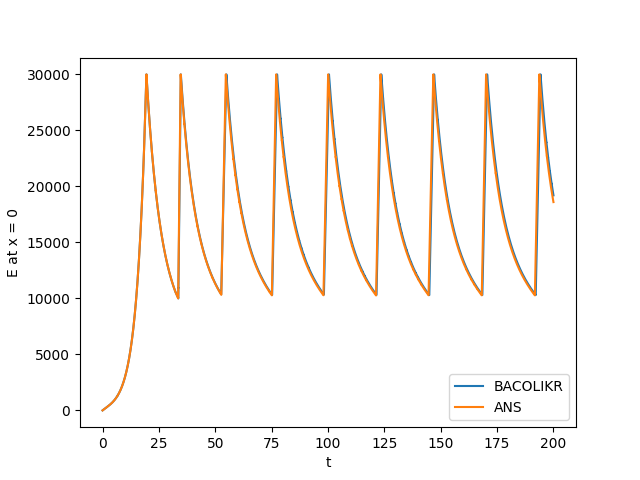
\includegraphics[width=0.7\linewidth]{./figures/pde_state_disc_event_tol_9}
\caption{Integral value plot of the event detection solution to state-dependent discontinuity problem with a tolerance of $10^{-9}$}
\label{fig:pde_state_disc_event_tol_9}
\end{figure}

We now note that both solutions even the one at $10^{-6}$ where much more accurate than the naive solution that was using manual fine-tuning of the time intervals, even the one with 1000 time intervals. Table $\ref{tab:pde_state_nfev}$ shows the number of function evaluations. 

\begin{table}[h]
\caption {PDE state discontinuity model} 
\label{tab:pde_state_nfev}
\begin{center}
\begin{tabular}{ c c } 
method                                & nfev \\ 
naive implementation with 400 steps   & 1, 184, 880   \\
naive implementation with 1000 steps  & 1, 280, 080    \\
naive implementation with 10000 steps & 1, 272, 030    \\
event detection at $10^{-6}$ tol.     & 1, 937, 730    \\
event detection at $10^{-9}$ tol.     & 7, 915, 085    \\
\end{tabular}
\end{center}
\end{table}

We note that the number of function evaluations is not the only measure of efficiency in this case as we also count the number of times the integration routine is called. We note that for the naive implementation, if we are using 'n' time intervals, then the integration routine is called n times. As for the event detection approach, the number of times the integration routine is called is the number of times the root function is called. With a tolerance of $10^{-6}$, the integration routine is called 2, 149 times and with a tolerance of $10^{-9}$, the integration routine is called 5, 059 times. We now note that the integration routine is thus called less than 10, 000 times in both cases and that the naive implementation did not get accurate enough even with 10, 000 calls to the integration routine. Thus event detection is the only way to get accurate solutions.

We also note that even with event detection, we are faced with a problem of finding a good trade-off between efficiency and accuracy. Improving the accuracy comes at the price of efficiency. In the next section we will perform a tolerance study to analyse this trade-off.

\subsubsection{State problem tolerance study}
\label{subsubsection:pde_state_tol_study}
In this section we perform a tolerance study on the case of using the naive implementation with a number of time intervals of 1000 and 10000 to see if using sharper tolerances allow us to get more accurate results. We also perform a tolerance study on the event detection solution to see show the efficiency and accuracy trade-off. We note that BACOLIKR even with event detection was facing a problem of not finding the exact location of the roots. The root-finding algorithm looked for zero up to some number of digits determined by the tolerance and thus at different tolerances, each root is detected at a slight offset. The offsets from consecutive roots compound into making the solution somewhat inaccurate at the later times. 

\paragraph{BACOLIKR without event}
\begin{figure}[H]
\centering
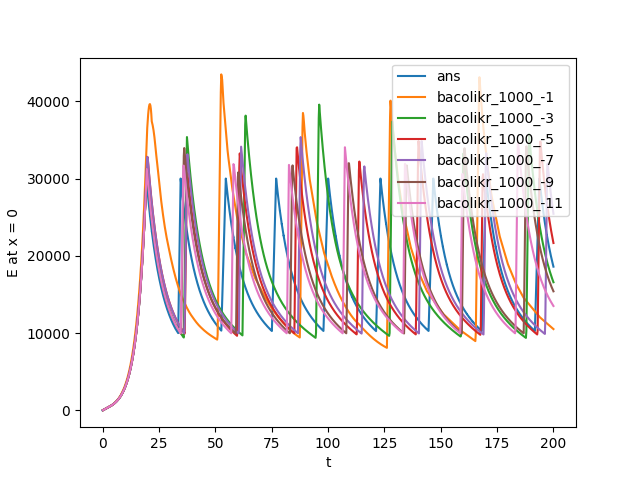
\includegraphics[width=0.7\linewidth]{./figures/pde_state_disc_tol_bacolikr_naive_1000}
\caption{Integral value plot of naive treatment to the state-dependent discontinuity problem at several tolerances using 1000 time intervals}
\label{fig:pde_state_disc_tol_bacolikr_naive_1000}
\end{figure}

\begin{figure}[H]
\centering
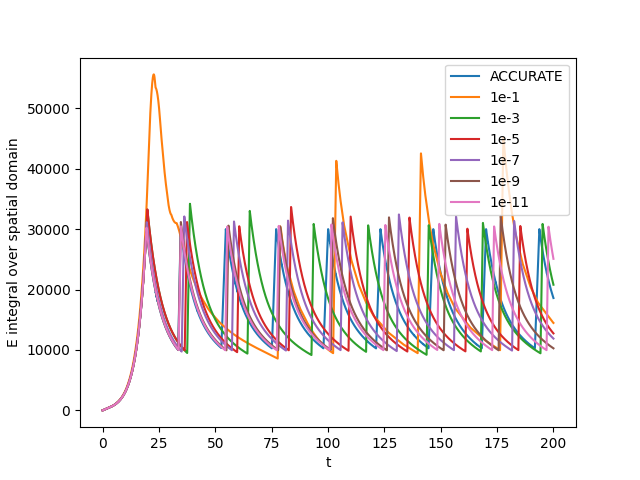
\includegraphics[width=0.7\linewidth]{./figures/pde_state_disc_tol_bacolikr_naive_10000}
\caption{Integral value plot of naive treatment to the state-dependent discontinuity problem at several tolerances using 10000 time intervals}
\label{fig:pde_state_disc_tol_bacolikr_naive_10000}
\end{figure}

Figures $\ref{fig:pde_state_disc_tol_bacolikr_naive_1000}$ and $\ref{fig:pde_state_disc_tol_bacolikr_naive_10000}$ show that the solutions at different tolerances with the naive implementation with 1000 and 10000 time intervals. We can see that increasing the number of time intervals does increase the accuracy of the solvers as with 10000 steps, the solutions oscillate more cleanly between 10000 and 30000. We note that in both cases, very coarse tolerances like $10^{-1}$ and $10^{-3}$ provide very erroneous solutions. Surprisingly, at really sharp tolerances like $10^{-9}$ and $10^{-11}$, the solutions are aligned with each others and with the answer for the first and going to the second root. However, even really sharp tolerances fail to remain accurate for long-term forecasts. See Table $\ref{tab:pde_state_tol_study}$ and Table $\ref{tab:pde_state_tol_num_integrations}$ for an idea of the efficiency comparison between using the naive implementation against using event detection.

\paragraph{BACOLIKR with event detection}
\begin{figure}[H]
\centering
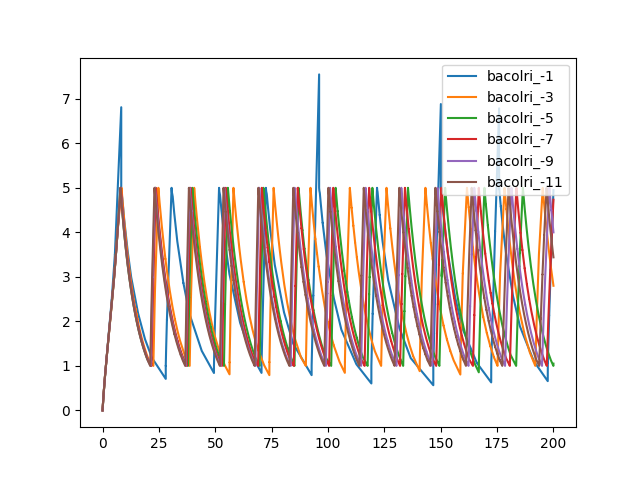
\includegraphics[width=0.7\linewidth]{./figures/pde_state_disc_tol_event}
\caption{Integral value plot of the event detection solution to state-dependent discontinuity problem at several tolerances}
\label{fig:pde_state_disc_tol_event}
\end{figure}

With event detection, the solution oscillate correctly for all tolerances except for $10^{-1}$ at the very first root. The other solutions are only slightly misaligned but this can be explained with the tolerance at the roots. Depending on the tolerance, the root is detected at a different location by the root-finding algorithm and thus different tolerances  detect the roots at slightly different offsets. These offsets compound such that the solutions are aligned for the first few roots but for longer term forecasts, a sharp tolerance is required. 

===============
We can potentially make the root finding / DASKR look for a root at a static tolerance, say 1e-6 and see what happens. This will help us confirm the above hypothesis/this can potentially be placed in 'future' works...
===============

\paragraph{Efficiency of the solvers}
\begin{table}[h]
\caption {State-dependent discontinuity number of function evaluations} 
\label{tab:pde_state_tol_study}
\begin{center}
\begin{tabular}{ c c c c } 
tolerance  & with event & naive 1000 intervals & naive 10000 intervals\\ 
1e-1       & 137, 300             & 101, 250            & 112, 600   \\
1e-3       & 376, 855             & 290, 600            & 343, 410   \\
1e-5       & 1, 052, 920          & 848, 080            & 862, 960  \\
1e-7       & 3, 217, 450          & 2, 217, 610         & 221, 5690   \\
1e-9       & 7, 915, 085          & 6, 040, 485         & 5, 811, 165  \\
1e-11      & 21, 256, 400         & 16, 402, 140        & 18, 508, 725  \\
\end{tabular}
\end{center}
\end{table}

\begin{table}[h]
\caption {Number of times the integration routine is called} 
\label{tab:pde_state_tol_num_integrations}
\begin{center}
\begin{tabular}{ c c } 
tolerance  & number of calls to integration routine \\ 
1e-1       &  420 \\
1e-3       &  940 \\
1e-5       & 1634 \\
1e-7       & 3405 \\
1e-9       & 5059 \\
1e-11      & 9753 \\
\end{tabular}
\end{center}
\end{table}

Table $\ref{tab:pde_state_tol_study}$ shows that we are forced to sacrifice efficiency for accuracy in this problem. We note that all naive solutions highly depend on the time stepping and thus should not be trusted for accurate solutions. Though they use less function evaluations than the event detection solutions of the same tolerance, we also note that for the case of 10000 time intervals and if we were to use even more time intervals, the integration routine is called less with event detection than with the naive implementation. Either way, the poor accuracy of the naive implementation of the solution to the state-dependent discontinuity problem should not be understated. Event detection is the only accurate way of solving such problems. 

For the solutions using event detection, the accuracy problem is at the roots where the models are to be changed. Depending on the tolerance, the root is detected at a different location as the root-finding algorithm returns the location of the root based on the tolerance. Thus different tolerances will lead to changing the models at slightly different positions. During the exponential increase phase, we can miss the location of the root by far enough that the solutions are not aligned.

\end{document}
